% ============================================================
%  J4 — APRÈS-MIDI : Transformers & Hugging Face
%  Julien Rolland — M2 Développement Fullstack
% ============================================================
\documentclass[aspectratio=169, 10pt]{beamer}
% ============================================================
%  PREAMBLE COMMUN — IA, Deep Learning & Machine Learning
%  Julien Rolland — M2 Développement Fullstack
% ============================================================

% --- Langue & encodage ---
\usepackage[utf8]{inputenc}
\usepackage[T1]{fontenc}
\usepackage{babel}
\babelprovide[import, main]{french}

% --- Thème Beamer ---
\usetheme{Madrid}
\usecolortheme{default}

% Palette de bleu académique
\definecolor{jedy_blue}{RGB}{0, 51, 102}       % bleu foncé principal
\definecolor{jedy_mid}{RGB}{0, 102, 179}        % bleu moyen accent
\definecolor{jedy_light}{RGB}{204, 221, 240}    % bleu très clair (fond boxes)
\definecolor{jedy_alert}{RGB}{180, 30, 30}      % rouge pour alertes
\definecolor{jedy_example}{RGB}{0, 120, 60}     % vert pour exemples

% Application des couleurs sur le thème Madrid
\setbeamercolor{palette primary}{bg=jedy_blue, fg=white}
\setbeamercolor{palette secondary}{bg=jedy_mid, fg=white}
\setbeamercolor{palette tertiary}{bg=jedy_blue, fg=white}
\setbeamercolor{palette quaternary}{bg=jedy_blue, fg=white}
\setbeamercolor{structure}{fg=jedy_blue}
\setbeamercolor{frametitle}{bg=jedy_blue, fg=white}
\setbeamercolor{title}{bg=jedy_blue, fg=white}
\setbeamercolor{block title}{bg=jedy_mid, fg=white}
\setbeamercolor{block body}{bg=jedy_light, fg=black}
\setbeamercolor{block title alerted}{bg=jedy_alert, fg=white}
\setbeamercolor{block body alerted}{bg=jedy_light, fg=black}
\setbeamercolor{block title example}{bg=jedy_example, fg=white}
\setbeamercolor{block body example}{bg=jedy_light, fg=black}

% --- Typographie ---
\usepackage{lmodern}
\setbeamerfont{title}{size=\Large, series=\bfseries}
\setbeamerfont{frametitle}{size=\normalsize, series=\bfseries}

% --- Navigation : suppression des icônes de navigation par défaut ---
\setbeamertemplate{navigation symbols}{}

% --- Numérotation des slides ---
\setbeamertemplate{footline}{%
  \leavevmode%
  \hbox{%
    \begin{beamercolorbox}[wd=.333\paperwidth,ht=2.25ex,dp=1ex,center]{author in head/foot}%
      \usebeamerfont{author in head/foot}\insertshortauthor
    \end{beamercolorbox}%
    \begin{beamercolorbox}[wd=.334\paperwidth,ht=2.25ex,dp=1ex,center]{title in head/foot}%
      \usebeamerfont{title in head/foot}\insertshorttitle
    \end{beamercolorbox}%
    \begin{beamercolorbox}[wd=.333\paperwidth,ht=2.25ex,dp=1ex,right]{date in head/foot}%
      \usebeamerfont{date in head/foot}
      \insertframenumber{} / \inserttotalframenumber\hspace*{2ex}
    \end{beamercolorbox}%
  }%
  \vskip0pt%
}

% --- Maths ---
\usepackage{amsmath, amssymb, amsthm}
\usepackage{bm}          % vecteurs en gras : \bm{w}

% --- Code source ---
\usepackage{listings}
\usepackage{xcolor}

\lstdefinestyle{pythonstyle}{
  language=Python,
  basicstyle=\ttfamily\footnotesize,
  keywordstyle=\color{jedy_blue}\bfseries,
  commentstyle=\color{gray}\itshape,
  stringstyle=\color{jedy_example},
  numberstyle=\tiny\color{gray},
  numbers=left,
  numbersep=5pt,
  frame=single,
  framerule=0.4pt,
  rulecolor=\color{jedy_light},
  backgroundcolor=\color{jedy_light!40},
  breaklines=true,
  showstringspaces=false,
  tabsize=4,
}
\lstset{style=pythonstyle}

% Alias pratique pour code inline
\newcommand{\code}[1]{\texttt{\small#1}}

% --- Graphiques ---
\usepackage{graphicx}
\usepackage{tikz}
\usetikzlibrary{arrows.meta, positioning, shapes.geometric, fit, calc}
\usepackage{pgfplots}
\pgfplotsset{compat=1.18}

% --- Tableaux ---
\usepackage{booktabs}
\usepackage{array}

% --- Icônes (optionnel, nécessite fontawesome5) ---
% \usepackage{fontawesome5}

% --- Macros ML/DL courantes ---
\newcommand{\R}{\mathbb{R}}
\newcommand{\E}{\mathbb{E}}
\newcommand{\Loss}{\mathcal{L}}
\newcommand{\dataset}{\mathcal{D}}
\newcommand{\X}{\mathbf{X}}
\newcommand{\y}{\mathbf{y}}
\newcommand{\w}{\mathbf{w}}
\newcommand{\W}{\mathbf{W}}
\newcommand{\grad}{\nabla}
\newcommand{\T}{^{\top}}         % transposée : \X\T
\newcommand{\lr}{\alpha}         % learning rate
\newcommand{\norm}[1]{\left\|#1\right\|}

% Encadré "Objectif pédagogique" en début de section
\newenvironment{objectif}{%
  \begin{alertblock}{Objectif}%
}{%
  \end{alertblock}%
}

% --- Infos du cours (remplacer dans chaque slides.tex) ---
\author[J. Rolland]{Julien Rolland}
\institute[Jedy]{Formation M2 Développement Fullstack}


\title[Transformers]{Transformers \& Hugging Face}
\subtitle{Jour 4 --- Après-midi}
\date{Jour 4}

% ============================================================
\begin{document}
% ============================================================

\begin{frame}
  \titlepage
\end{frame}

\begin{frame}{Plan du module}
  \tableofcontents
\end{frame}

% ============================================================
\section{Du contexte à l'attention}
% ============================================================

\begin{frame}{Le problème du contexte}
  \begin{columns}[T]
    \begin{column}{0.50\textwidth}
      \begin{alertblock}{La polysémie en pratique}
        \begin{itemize}
          \item «~La \textbf{souris} mange le fromage.~»
          \item «~Ma \textbf{souris} d'ordinateur est cassée.~»
        \end{itemize}
        \vspace{4pt}
        Dans Word2Vec, «~souris~» n'a \textbf{qu'un seul vecteur}
        --- une moyenne des deux sens.
      \end{alertblock}
      \smallskip
      \begin{block}{Les autres limites (rappel J4-AM)}
        \begin{itemize}
          \item Embeddings \textbf{figés} après entraînement
          \item Ignorent l'\textbf{ordre} des mots dans la phrase
          \item Biais hérités du corpus d'entraînement
        \end{itemize}
      \end{block}
    \end{column}
    \begin{column}{0.46\textwidth}
      \begin{exampleblock}{Le besoin : embeddings contextuels}
        Le vecteur d'un mot doit être calculé
        \textbf{à la volée} en fonction de ses voisins.
        \vspace{4pt}
        \begin{center}
          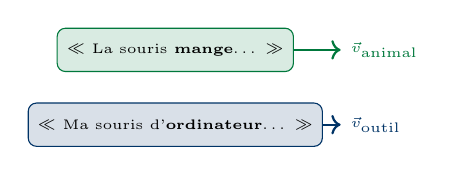
\begin{tikzpicture}[font=\tiny,
            box/.style={draw, rounded corners=3pt, align=center,
                        minimum width=3.0cm, minimum height=0.55cm}]
            \node[box, fill=jedy_example!15, draw=jedy_example] (b1) at (0,0)
              {«~La souris \textbf{mange}\ldots~»};
            \node[box, fill=jedy_blue!15, draw=jedy_blue] (b2) at (0,-0.95)
              {«~Ma souris d'\textbf{ordinateur}\ldots~»};
            \draw[->, jedy_example, thick] (b1.east) -- (2.1, 0.0)
              node[right] {$\vec{v}_{\text{animal}}$};
            \draw[->, jedy_blue, thick] (b2.east) -- (2.1,-0.95)
              node[right] {$\vec{v}_{\text{outil}}$};
          \end{tikzpicture}
        \end{center}
      \end{exampleblock}
      \vspace{2pt}
      \begin{alertblock}{Solution}
        Le \textbf{mécanisme d'attention} --- cœur du Transformer.
      \end{alertblock}
    \end{column}
  \end{columns}
\end{frame}

\begin{frame}{L'intuition de l'attention}
  \begin{columns}[T]
    \begin{column}{0.52\textwidth}
      \begin{exampleblock}{Principe \& exemple}
        Chaque mot «~vote~» pour ceux qui l'aident à se définir.\\[2pt]
        «~L'animal \ldots\ car \textbf{il} était fatigué.~»\\[2pt]
        Distribution d'attention de «~il~» :
        \begin{itemize}
          \item \textbf{animal} : \textbf{90\,\%}
          \item fatigué : 6\,\%
          \item autres mots : 4\,\%
        \end{itemize}
      \end{exampleblock}
      \vspace{2pt}
      \begin{alertblock}{Avantage : parallélisme}
        Contrairement aux RNN, l'attention traite
        \textbf{tous les mots simultanément} --- GPU.
      \end{alertblock}
    \end{column}
    \begin{column}{0.44\textwidth}
      \begin{block}{Distribution d'attention de «~\textbf{il}~»}
        \begin{itemize}
          \item[\textcolor{jedy_alert}{\textbf{90\,\%}}]
                \textbf{animal} --- co-référence directe
          \item[\textcolor{jedy_mid}{6\,\%}]
                \textbf{fatigué} --- trait partagé
          \item[4\,\%] autres mots (négligeable)
        \end{itemize}
      \end{block}
      \vspace{2pt}
      \begin{exampleblock}{Interprétation}
        Le modèle «~sait~» que «~il~» réfère à «~animal~»
        \textbf{grâce au contexte} global --- sans règle
        grammaticale explicite.
      \end{exampleblock}
    \end{column}
  \end{columns}
\end{frame}

\begin{frame}{La formule de l'attention}
  \begin{columns}[T]
    \begin{column}{0.52\textwidth}
      \begin{block}{Mécanisme Query / Key / Value}
        \begin{itemize}
          \item $Q$ (\textit{Query}) : «~Ce que je \textbf{cherche}.~»
          \item $K$ (\textit{Key}) : «~Ce que j'\textbf{offre}.~»
          \item $V$ (\textit{Value}) : «~L'information que je \textbf{contiens}.~»
        \end{itemize}
      \end{block}
      \smallskip
      \begin{block}{Équation}
        \[
          \mathrm{Attention}(Q,K,V)
          = \mathrm{softmax}\!\left(\frac{QK^{\T}}{\sqrt{d_k}}\right)V
        \]
        \begin{itemize}
          \item $QK^{\T}$ : score de pertinence (mot, mot)
          \item $\sqrt{d_k}$ : normalisation (gradients stables)
          \item Softmax $\to$ poids $\in [0,1]$, somme $= 1$
        \end{itemize}
      \end{block}
    \end{column}
    \begin{column}{0.44\textwidth}
      \begin{exampleblock}{Multi-Head Attention}
        On lance $h$ attentions en \textbf{parallèle}
        sur des sous-espaces distincts :
        \begin{itemize}
          \item Tête 1 : relations \textbf{grammaticales}
          \item Tête 2 : relations \textbf{sémantiques}
          \item Tête 3 : relations de \textbf{coréférence}
          \item \ldots
        \end{itemize}
        \vspace{4pt}
        Les sorties sont \textbf{concaténées} puis projetées.
      \end{exampleblock}
      \vspace{2pt}
      \begin{alertblock}{Note «~Geek~»}
        C'est une \textbf{recherche floue} dans une base de données
        vectorielle : $Q$ est la requête, $K$ l'index, $V$ le résultat.
      \end{alertblock}
    \end{column}
  \end{columns}
\end{frame}

% ============================================================
\section{L'architecture Transformer}
% ============================================================

\begin{frame}{Encoder, Decoder, Seq2Seq}
  \begin{columns}[T]
    \begin{column}{0.31\textwidth}
      \begin{block}{Encoder (ex: BERT)}
        \begin{itemize}
          \item[\textcolor{jedy_example}{$+$}] Lit la phrase
                \textbf{dans les deux sens}
          \item[\textcolor{jedy_example}{$+$}] Embeddings contextuels
                riches
          \item Idéal : \textbf{classification},
                NER, question-answering
        \end{itemize}
      \end{block}
    \end{column}
    \begin{column}{0.31\textwidth}
      \begin{block}{Decoder (ex: GPT)}
        \begin{itemize}
          \item[\textcolor{jedy_example}{$+$}] Génère mot après mot
                (\textit{autoregressive})
          \item Attention \textbf{masquée} : ne voit que le passé
          \item Idéal : \textbf{génération} de texte, chatbots
        \end{itemize}
      \end{block}
    \end{column}
    \begin{column}{0.31\textwidth}
      \begin{block}{Encoder-Decoder (ex: T5)}
        \begin{itemize}
          \item[\textcolor{jedy_example}{$+$}] Encode la source,
                décode la cible
          \item Idéal : \textbf{traduction},
                résumé, reformulation
        \end{itemize}
      \end{block}
    \end{column}
  \end{columns}
  \medskip
  \begin{center}
    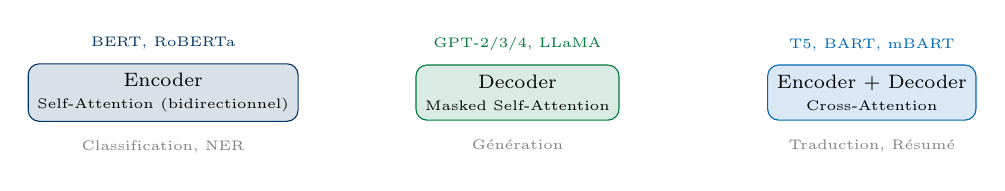
\begin{tikzpicture}[font=\scriptsize,
      blk/.style={draw, rounded corners=4pt, align=center,
                  minimum width=2.4cm, minimum height=0.7cm},
      arr/.style={->, thick, gray!60}]
      % Encoder
      \node[blk, fill=jedy_blue!15, draw=jedy_blue] (enc)
        at (0,0) {Encoder\\{\tiny Self-Attention (bidirectionnel)}};
      \node[above=0.05cm of enc, font=\tiny, color=jedy_blue]
        {BERT, RoBERTa};
      % Decoder
      \node[blk, fill=jedy_example!15, draw=jedy_example] (dec)
        at (4.5,0) {Decoder\\{\tiny Masked Self-Attention}};
      \node[above=0.05cm of dec, font=\tiny, color=jedy_example]
        {GPT-2/3/4, LLaMA};
      % Seq2Seq
      \node[blk, fill=jedy_mid!15, draw=jedy_mid] (s2s)
        at (9.0,0) {Encoder + Decoder\\{\tiny Cross-Attention}};
      \node[above=0.05cm of s2s, font=\tiny, color=jedy_mid]
        {T5, BART, mBART};
      % Étiquettes tâche
      \node[below=0.12cm of enc, font=\tiny, color=gray]
        {Classification, NER};
      \node[below=0.12cm of dec, font=\tiny, color=gray]
        {Génération};
      \node[below=0.12cm of s2s, font=\tiny, color=gray]
        {Traduction, Résumé};
    \end{tikzpicture}
  \end{center}
\end{frame}

\begin{frame}{Le paradigme du Transfer Learning}
  \begin{columns}[T]
    \begin{column}{0.50\textwidth}
      \begin{alertblock}{Pre-training --- la fondation}
        \begin{itemize}
          \item Entraînement massif sur \textbf{tout Internet}
                (Wikipédia, livres, code\ldots)
          \item Objectif : \textbf{prédire le token masqué} (BERT)
                ou le token suivant (GPT)
          \item Coût : millions d'euros de calcul GPU
          \item Résultat : le modèle apprend la \textbf{«~langue~»}
                --- grammaire, faits, raisonnement
        \end{itemize}
      \end{alertblock}
    \end{column}
    \begin{column}{0.46\textwidth}
      \begin{exampleblock}{Fine-tuning --- l'adaptation}
        On ajuste le modèle sur une \textbf{tâche métier} :
        \begin{itemize}
          \item Classification de tickets support
          \item Résumé automatique de rapports
          \item Détection de sentiment client
        \end{itemize}
        \vspace{4pt}
        \textbf{Quelques dizaines de lignes} de code,
        quelques \textbf{minutes} de calcul $\to$
        niveau état de l'art.
      \end{exampleblock}
      \smallskip
      \begin{block}{Pourquoi ça marche ?}
        Les couches inférieures encodent des
        connaissances \textbf{générales} réutilisables ;
        seule la tête de classification change.
      \end{block}
    \end{column}
  \end{columns}
\end{frame}

% ============================================================
\section{Hugging Face en pratique}
% ============================================================

\begin{frame}{L'écosystème Hugging Face}
  \begin{columns}[T]
    \begin{column}{0.48\textwidth}
      \begin{block}{The Hub}
        Le «~GitHub~» des modèles d'IA :
        \begin{itemize}
          \item $> 100\,000$ modèles prêts à l'emploi
          \item Hébergement gratuit des poids
          \item Versionning, fiches modèles,
                benchmarks intégrés
        \end{itemize}
      \end{block}
      \smallskip
      \begin{block}{\texttt{datasets}}
        \begin{itemize}
          \item Accès instantané à des milliers de
                bases de données (IMDb, Wikipedia,
                GLUE, SQuAD\ldots)
          \item Chargement en une ligne :
          \item[] \quad\texttt{\small load\_dataset("imdb")}
        \end{itemize}
      \end{block}
    \end{column}
    \begin{column}{0.48\textwidth}
      \begin{exampleblock}{\texttt{transformers}}
        Interface \textbf{unifiée} pour tout modèle :
        \begin{itemize}
          \item BERT, RoBERTa, CamemBERT
          \item GPT-2, LLaMA, Mistral
          \item T5, BART, Whisper, CLIP\ldots
        \end{itemize}
        Même API quel que soit l'architecture.
      \end{exampleblock}
      \smallskip
      \begin{alertblock}{Écosystème complet}
        \begin{itemize}
          \item \texttt{tokenizers} : tokeniseurs rapides (Rust)
          \item \texttt{evaluate} : métriques standardisées
          \item \texttt{accelerate} : multi-GPU/TPU
          \item \texttt{PEFT} : fine-tuning efficace (LoRA)
        \end{itemize}
      \end{alertblock}
    \end{column}
  \end{columns}
\end{frame}

\begin{frame}[fragile]{La \texttt{pipeline} API --- le mode «~Product~»}
  \begin{columns}[T]
    \begin{column}{0.52\textwidth}
      \begin{block}{Concept}
        Abstraction totale : téléchargement du modèle,
        tokenisation, inférence, décodage --- tout en
        \textbf{une seule ligne}.
      \end{block}
      \smallskip
\begin{lstlisting}[language=Python]
from transformers import pipeline

clf = pipeline("sentiment-analysis")
print(clf("Ce cours est dense !"))
# [{'label':'POSITIVE', 'score':0.98}]

trad = pipeline("translation",
    model="Helsinki-NLP/opus-mt-fr-en")
print(trad("Bonjour le monde"))
# [{'translation_text':'Hello World'}]
\end{lstlisting}
    \end{column}
    \begin{column}{0.44\textwidth}
      \begin{exampleblock}{Tâches disponibles}
        \begin{itemize}
          \item \texttt{"sentiment-analysis"}
          \item \texttt{"text-generation"}
          \item \texttt{"summarization"}
          \item \texttt{"translation"}
          \item \texttt{"question-answering"}
          \item \texttt{"ner"} (entités nommées)
        \end{itemize}
      \end{exampleblock}
      \vspace{2pt}
      \begin{alertblock}{Intérêt terrain}
        C'est ce qu'un dev Fullstack utilisera
        \textbf{90\,\% du temps} en entreprise.
        Pas besoin de connaître l'architecture interne.
      \end{alertblock}
    \end{column}
  \end{columns}
\end{frame}

\begin{frame}[fragile]{Anatomie du Fine-Tuning --- le mode «~Expert~»}
  \begin{columns}[T]
    \begin{column}{0.52\textwidth}
      \begin{block}{Les 3 composants obligatoires}
        \begin{enumerate}
          \item \textbf{Tokenizer} : identique au modèle pré-entraîné
          \item \textbf{Model Head} : couche de sortie remplacée
                (ex: $30\,000 \to 2$ classes)
          \item \textbf{Trainer} : boucle d'entraînement optimisée
        \end{enumerate}
      \end{block}
      \vspace{2pt}
\begin{lstlisting}[language=Python]
from transformers import (
    AutoTokenizer,
    AutoModelForSequenceClassification,
)
model = AutoModelForSequenceClassification\
  .from_pretrained("camembert-base",
                   num_labels=2)
tokenizer = AutoTokenizer\
  .from_pretrained("camembert-base")
\end{lstlisting}
    \end{column}
    \begin{column}{0.44\textwidth}
      \begin{exampleblock}{Pourquoi le Tokenizer doit coïncider ?}
        Le modèle a appris des embeddings pour des IDs
        précis. Si l'on utilise un tokenizer différent,
        les IDs ne correspondent plus aux poids ---
        le modèle produit du bruit.
      \end{exampleblock}
      \vspace{2pt}
      \begin{block}{Alternatives légères}
        \begin{itemize}
          \item \textbf{LoRA / QLoRA} : $< 1\,\%$ des params
          \item \textbf{Prompt-tuning} : tokens «~soft~»
          \item \textbf{Zero-shot} : sans fine-tuning
        \end{itemize}
      \end{block}
    \end{column}
  \end{columns}
\end{frame}

% ============================================================
\section{Évaluation}
% ============================================================

\begin{frame}{Évaluation : au-delà de l'accuracy}
  \begin{columns}[T]
    \begin{column}{0.50\textwidth}
      \begin{alertblock}{Pourquoi l'accuracy ment}
        99\,\% de mails normaux, 1\,\% de spams.\\[2pt]
        Prédire «~normal~» partout $\to$ \textbf{99\,\%} ---
        mais le modèle est \textbf{inutile}.
      \end{alertblock}
      \smallskip
      \begin{block}{Précision \& Rappel}
        \vspace{2pt}
        $\displaystyle\text{Précision} = \dfrac{TP}{TP{+}FP}$
        \qquad
        $\displaystyle\text{Rappel} = \dfrac{TP}{TP{+}FN}$
        \vspace{2pt}
      \end{block}
      \smallskip
      \begin{exampleblock}{F1-Score --- moyenne harmonique}
        \[
          F_1 = 2 \cdot
          \frac{\text{Précision} \times \text{Rappel}}
               {\text{Précision} + \text{Rappel}}
        \]
      \end{exampleblock}
    \end{column}
    \begin{column}{0.46\textwidth}
      \begin{block}{Matrice de confusion}
        Visualiser \textbf{où} le modèle se trompe :
        \vspace{2pt}
        \begin{center}
          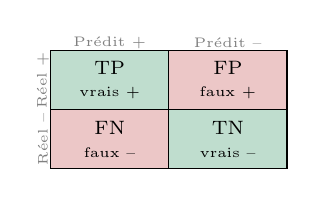
\begin{tikzpicture}[font=\scriptsize]
            \node[draw, fill=jedy_example!25,
                  minimum width=1.5cm, minimum height=0.75cm, align=center,
                  font=\scriptsize] at (0.75, -0.375)  {TP\\{\tiny vrais +}};
            \node[draw, fill=jedy_alert!25,
                  minimum width=1.5cm, minimum height=0.75cm, align=center,
                  font=\scriptsize] at (2.25, -0.375)  {FP\\{\tiny faux +}};
            \node[draw, fill=jedy_alert!25,
                  minimum width=1.5cm, minimum height=0.75cm, align=center,
                  font=\scriptsize] at (0.75, -1.125)  {FN\\{\tiny faux --}};
            \node[draw, fill=jedy_example!25,
                  minimum width=1.5cm, minimum height=0.75cm, align=center,
                  font=\scriptsize] at (2.25, -1.125)  {TN\\{\tiny vrais --}};
            \node[font=\tiny, color=gray] at (0.75,  0.1)  {Prédit +};
            \node[font=\tiny, color=gray] at (2.25,  0.1)  {Prédit --};
            \node[font=\tiny, color=gray, rotate=90] at (-0.1,-0.375) {Réel +};
            \node[font=\tiny, color=gray, rotate=90] at (-0.1,-1.125) {Réel --};
          \end{tikzpicture}
        \end{center}
      \end{block}
      \vspace{2pt}
      \begin{alertblock}{Exemple}
        Confondre «~colère~» et «~tristesse~» est moins grave
        que «~positif~» et «~négatif~» --- la matrice le révèle.
      \end{alertblock}
    \end{column}
  \end{columns}
\end{frame}

\end{document}
